\chapter{Interactive Visual Odometry on the Web}%
\label{cha:interactive_vo_on_the_web}

\minitoc%
\clearpage

\section{Visual Odometry in Rust (VORS)}%
\label{sec:vors}

\subsection{Overview of VORS}%
\label{sub:vors-overview}

VORS is a sparse, keyframe-based, RGB-D, direct visual odometry algorithm.
As presented in Section~\ref{sub:appearance-based},
VORS belongs to the family of direct visual odometry,
based on the image alignment optimization problem.
Contrary to monocular visual odometry, which requires an estimation
of points depth, we focus on the RGB-D case,
where the necessary depth information for reprojection is provided by a sensor.
In order to reduce drift when the camera moves slowly,
image alignment is performed from a fixed keyframe instead of the previous frame.
Decision to change the keyframe is done heuristically;
details are presented in Section~\ref{sub:multi-res-direct-image-alignment}.
Finally, our algorithm uses a sparse subset of points in the image,
which has been shown~\cite{engel2017direct} to be sufficient to track the camera motion.
Disregarding sparsity and robustness, discussed later,
our algorithm is very similar to DVO~\cite{kerl2013robust},
and its predecessor~\cite{steinbrucker2011real}.
An overview of the full pipeline of VORS is presented in Figure~\ref{fig:overview-vors}.

\begin{figure}[ht]
	\centering
	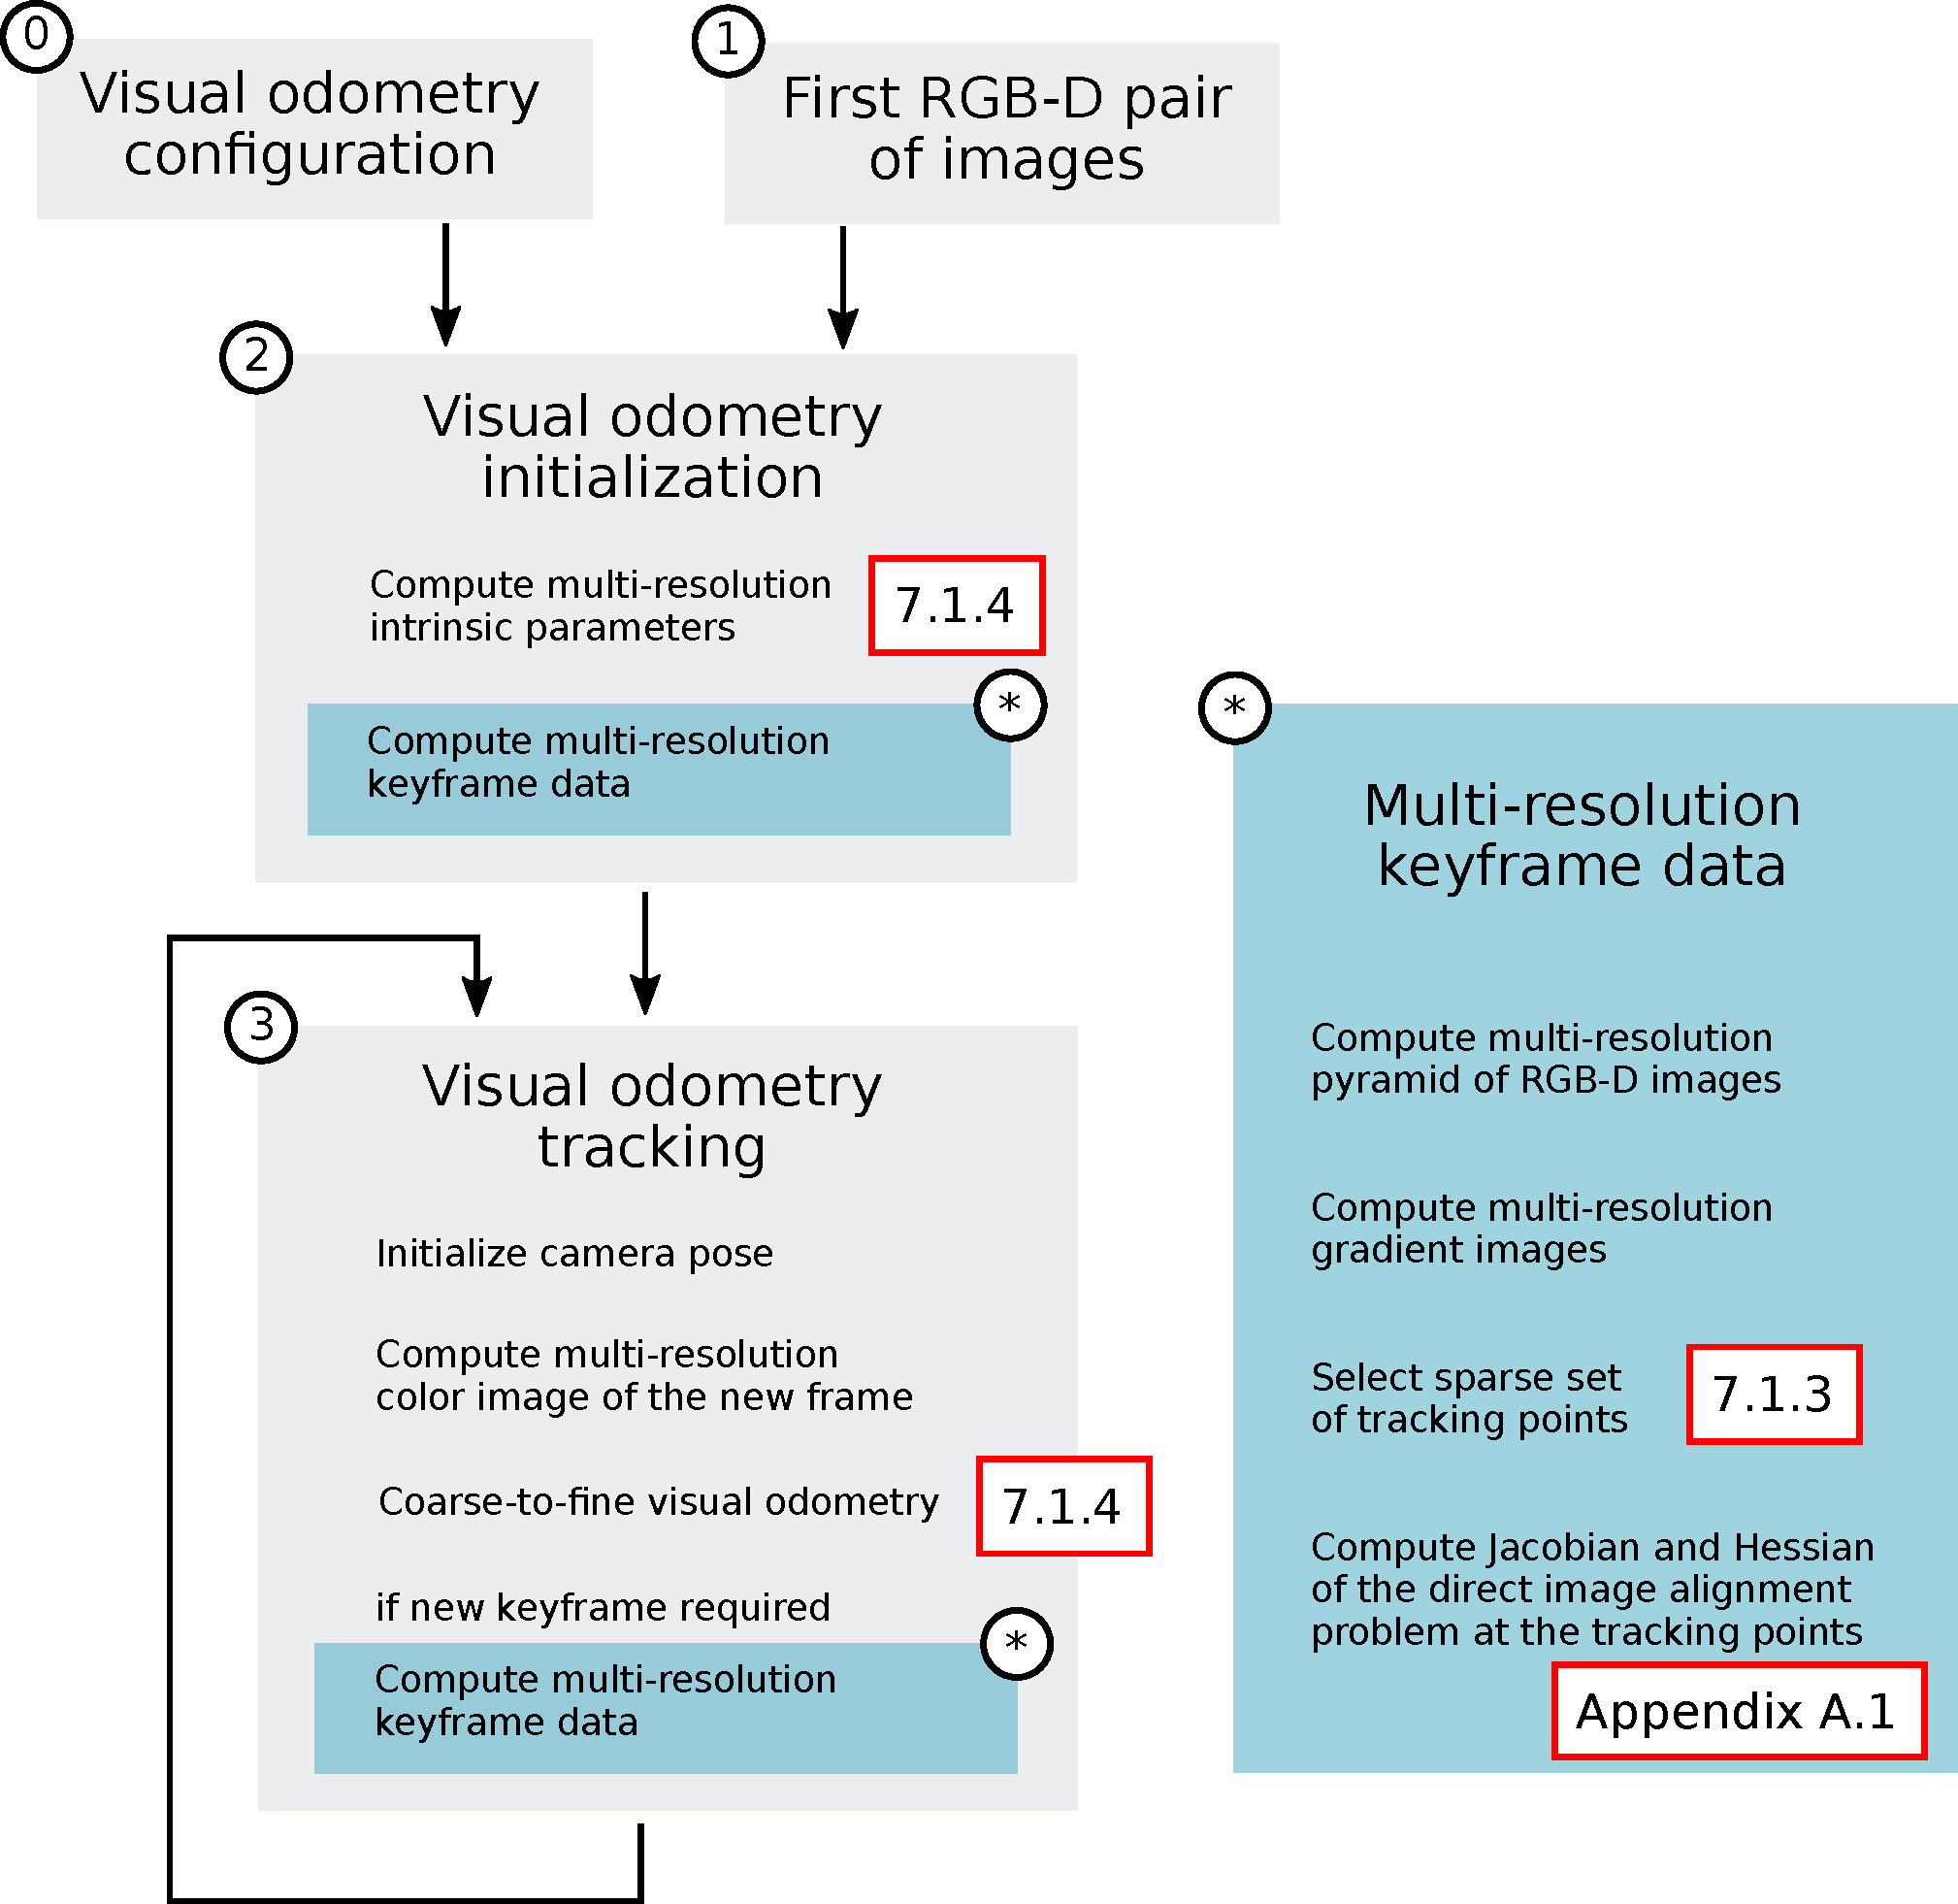
\includegraphics[width=\linewidth]{assets/img/overview-vors.pdf}
	\caption{Overview of VORS pipeline.}%
	\label{fig:overview-vors}
\end{figure}

\subsection{Sparse Points Selection}%
\label{sub:sparse-points}

Engel et al.\ demonstrated in DSO~\cite{engel2017direct} that using a sparse subset
of points for the direct image alignment problem still results in precise camera locations
at the condition that points satisfy two conditions,
\begin{itemize}
\setlength\itemsep{-0.5em}
	\item they should be well distributed in the image,
	\item and they should be located at positions with higher gradients magnitudes.
\end{itemize}
Selected points are called candidate points,
and their selection mechanism is rather complex, based on at least ten parameters.
The core idea is to regularly divide an image in tiles.
One subdivision produces big tiles, called regions,
and another generates small tiles, called blocks.
One pixel is selected per block if its gradient is higher than a local threshold
depending on the region containing the pixel.
In practice, blocks are actually multi-scale, with three default levels.
If none of the four ``level $n$'' blocks composing a ``level $(n+1)$'' block elected a candidate point,
the ``level $(n+1)$'' block checks whether a pixel satisfies a lower threshold.
The factor between block thresholds at different levels is one of the parameters.
Another mechanism aims at obtaining a target amount of candidate points.
That amount can be approximated from blocks base size but it might differ.
Depending on the difference with the target count,
the algorithm will choose between the three following options,
(1) keep candidates, (2) randomly select a sample of the candidates,
or (3) change the block base size and restart from scratch.

In contrast, our sparse selection of candidates is rather simple,
based on a multi-resolution pyramid of images.
We embraced the idea that each level of the image pyramid should exhibit
that property of well distributed points with higher density near higher gradients.
% Intuitively, it should help convergence of the alignment problem to a global minimum.
We thus propose a simple coarse-to-fine selection mechanism,
depicted in Figure~\ref{fig:coarse-to-fine-candidates}.
At the lowest resolution, all points are candidates.
For each candidate pixel at one pyramid level, we elect one or two candidates
in the four subpixels of the next level.
A threshold based on gradients is used to determine which pixels should be selected.
This sparse selection scheme ensures that there is at least one candidate per region
corresponding to one pixel at the lowest resolution.
It also increases the density of candidates in higher gradients areas.
The number of levels of the image pyramid is a common parameter for candidates selection
and for the multi-resolution direct image alignement presented next.

\begin{figure}[ht]
	\centering
	
\includegraphics[width=0.23\linewidth]{assets/img/candidates-icl-4.png}
	\hfill
	
\includegraphics[width=0.23\linewidth]{assets/img/candidates-icl-3.png}
	\hfill
	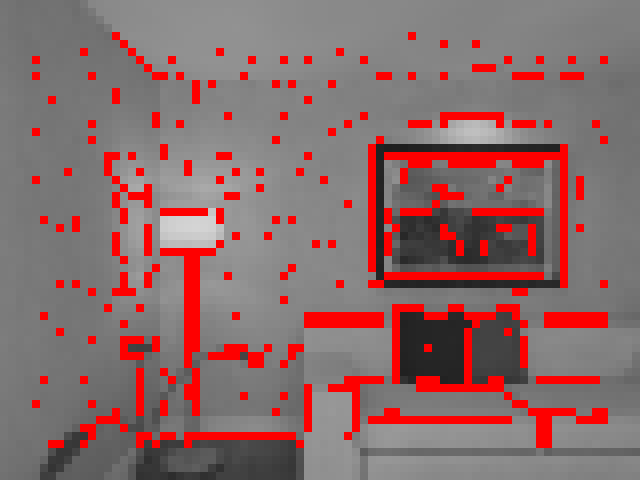
\includegraphics[width=0.23\linewidth]{assets/img/candidates-icl-2.png}
	\hfill
	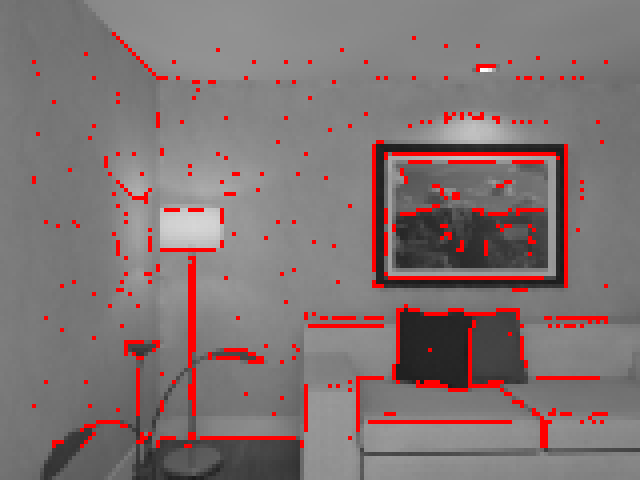
\includegraphics[width=0.23\linewidth]{assets/img/candidates-icl-1.png}
	\caption{Coarse-to-fine candidate selection of VORS.
	Candidates are represented in red.
	All points are kept at the lowest resolution.
	Each higher resolution elects one or two candidates per parent candidate.}%
	\label{fig:coarse-to-fine-candidates}
\end{figure}

Figure~\ref{fig:candidates-dso-vors} depicts a zoomed-in view of the same image region
for both DSO and VORS candidates selection mechanisms.
As visible on the left image, DSO candidate points are regularly spaced,
except in homogenous areas.
VORS candidate points however tend to form contiguous lines,
which probably generates redundant information.
Limiting the maximum number of subpixel candidates to one
at some levels (in the higher resolutions),
could both help control the maximum amount of candidates and
limit the information redundancy generated by neighbour candidates.

\begin{figure}[t]
	\centering
	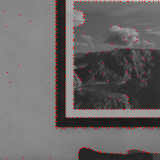
\includegraphics[width=0.49\linewidth]{assets/img/candidates-icl-dso-cropped.png}
	\hfill
	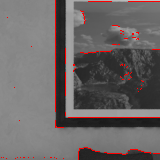
\includegraphics[width=0.49\linewidth]{assets/img/candidates-icl-vors-cropped.png}
	\caption{DSO (left) and VORS (right) candidate points (in red).}%
	\label{fig:candidates-dso-vors}
\end{figure}

\subsection{Multi-Resolution Direct Image Alignment}%
\label{sub:multi-res-direct-image-alignment}

\subsubsection{Convergence of the Optimization Problem}%
\label{ssub:convergence-optimization}

As presented in Section~\ref{sub:appearance-based},
under the photoconsistency assumption, direct image alignment consists
in finding the warp function $W$ minimizing
\[
	\sum_{\bm{x}}\|I(W(\bm{x})) - I^{*}(\bm{x})\|^2
\]
where $I^{*}, I$ are the reference and new images,
and $\bm{x}$ is the position of a pixel in the reference image.
As explained in Baker and Matthews~\cite{baker2004lucas},
this can be minimized with an iterative optimization.
If we note $\bm{\xi}$ the parameters of the warp function,
and $\delta\bm{\xi}$ the iterative increments,
the expression of the residual in an inverse compositional formulation is
\[
	I^{*}(W(\bm{x}, \delta \bm{\xi})) - I(W(\bm{x}, \bm{\xi})).
\]
In a Gauss-Newton scheme, the iterative increment $\delta\bm{\xi}$ is computed as
\[
	\delta \bm{\xi} = \inv{H} \sum_{\bm{x}} \tr{J} (I^{*}(\bm{x}) - I(W(\bm{x}, \bm{\xi})))
\]
where $J = \nabla I \cdot J_{\bm{\xi}}W$, $\nabla I$ is the image gradient
and $J_{\bm{\xi}}W$ is the Jacobian of the warp function.
The Hessian is computed as the Gauss-Newton approximation
$H = \sum_{\bm{x}}\tr{J}J$.
We parameterize $W$ in the Lie algebra of twists $\seee$.
The expression of the Jacobian of the warp function
is detailed in Appendix~\ref{sec:notation}.

In theory however, this iterative algorithm is only correct under the assumption
that the initialization is already near the solution.
Convergence to the correct minimum is thus a hard problem
and under some circumstances, the optimization may drift to another local minimum.
One way to help convergence is to use the Levenberg-Marquardt approximation
of the Hessian.
It consists in multiplying the diagonal elements of
the Gauss-Newton approximation of the Hessian by $(1 + \lambda_{lm})$.
The Levenberg-Marquardt coefficient $\lambda_{lm}$ is dynamically
updated toward 0 when converging or toward $+\infty$ when diverging.

Another method to improve convergence consists in solving the optimization
with a coarse-to-fine multi-resolution approach.
Indeed, the image gradient used for the Jacobian contains information
of larger areas of the original image when computed at lower resolutions.
As a consequence, the vicinity of the global optimum is artificially increased.
For the direct image alignment, we thus use a pyramid of images,
where each level has half the resolution of the previous one.
As explained previously the number of levels also impacts candidate points selection.
Indeed, at the lowest resolution, all pixels serve as candidates for the optimization.
The number of levels is thus chosen as a compromise between the minimum amount
of candidate points and the desired convergence rate.
Starting from 640x480 images in the ICL-NUIM and TUM RGB-D datasets,
we found that 6 levels is a good compromise.
The lowest resolution has 20x15 images, which implies a minimum of 300 candidate points.

\subsubsection{Multi-Resolution Intrinsics}%
\label{ssub:multires-intrinsics}

Since we use a coarse-to-fine optimization,
we must be able to initialize one level from the result of the previous one.
In Section~\ref{sub:intrinsic_parameters}, we presented the image formation as
the succession of two transformations, first the projection from the camera frame
to the image frame, and then the projection onto the pixels frame.
When halving the image resolution, the second transformation $K_s$ changes.
\[
	K_s = \begin{pmatrix}
		s_x & s_{\theta} & o_x \\
		0 & s_y & o_y \\
		0 & 0 & 1 \\
	\end{pmatrix}.
\]
We note $K_s'$ the new pixels projection with a resolution multiplied by $\alpha$.
In our case $\alpha$ is of the form $2^{-n}$.
On the one hand, scaling parameters are all multiplied by $\alpha$ i.e.\
$s_x' = \alpha s_x$,
$s_y' = \alpha s_y$ and
$s_{\theta}' = \alpha s_{\theta}$.
The principal point parameters on the other hand depend on the origin of the coordinate system.
In most modelizations, the value of pixel $(x,y)$ is interpreted as the integration
of the light hitting the sensor on the surface located between $(x-0.5, y-0.5)$
and $(x+0.5, y+0.5)$.
The coordinates of the top left corner of the image is thus $(-0.5, -0.5)$
instead of $(0,0)$.
Figure~\ref{fig:multiscale-intrinsics} illustrates how
the principal point is transformed in such coordinate system.
As a result, the location of the principal point is updated as
$o_x' = \alpha(o_x + 0.5) - 0.5$ and
$o_y' = \alpha(o_y + 0.5) - 0.5$.
In the end, the updated intrinsic pixel transformation is
\[
	K_s' = K_{\alpha}K_s \quad \text{with} \quad
	K_{\alpha} = \begin{pmatrix}
		\alpha & 0 & 0.5(\alpha - 1) \\
		0 & \alpha & 0.5(\alpha - 1) \\
		0 & 0 & 1 \\
	\end{pmatrix}.
\]

\begin{figure}[t]
	\centering
	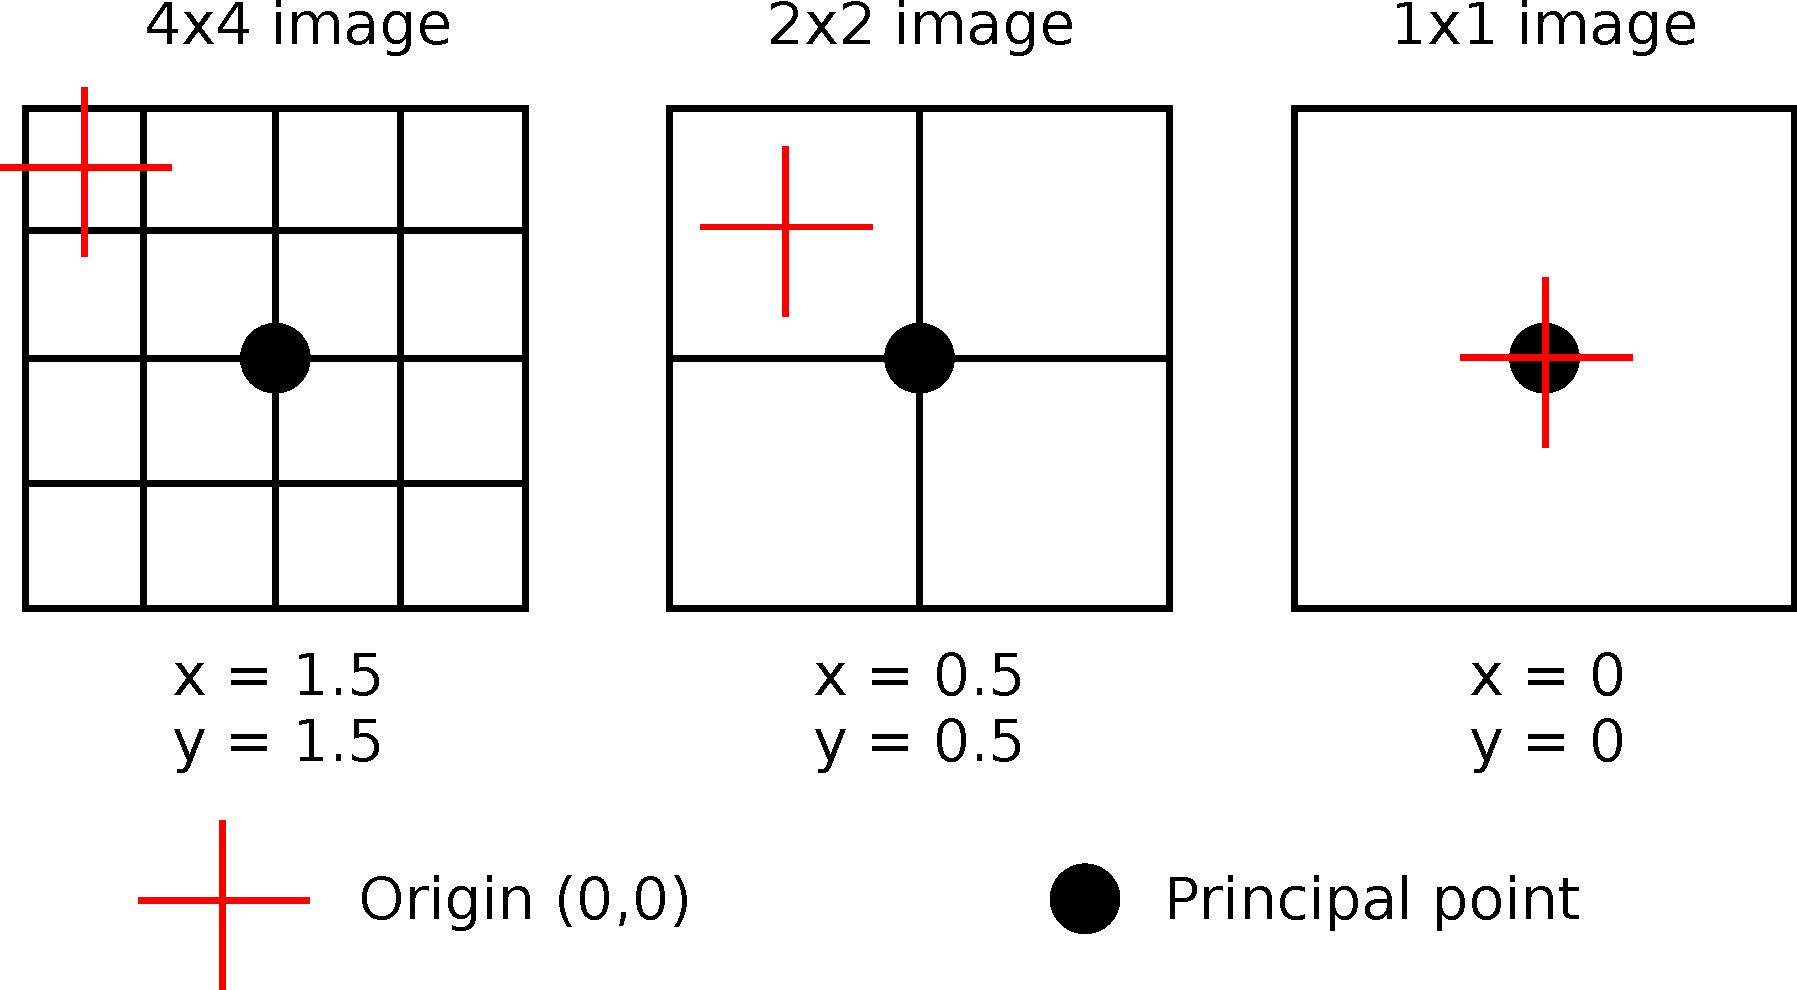
\includegraphics[width=\linewidth]{assets/img/multiscale-intrinsics.pdf}
	\caption{Effect of a centered coordinate system on
	the coordinates of the principal point at multiple resolutions.}%
	\label{fig:multiscale-intrinsics}
\end{figure}

The presented approach is the one used by the TUM RGB-D coordinate system
for the principal point given in the intrinsics matrix.
It is thus also the one we use when initializing the multi-resolution intrinsic
parameters in step 2 of Figure~\ref{fig:overview-vors}.
The camera motion estimated at one resolution can thus be reused as-is
for the initialization of the next resolution.
It is the projection that changes, due to a different intrinsic matrix.

\subsubsection{Keyframe Update}%
\label{ssub:keyframe-update}

We mentioned in VORS overview that the decision to change the keyframe is done heuristically.
Similarly to ORB-SLAM~\cite{mur2015orb} and DSO~\cite{engel2017direct},
we use the optical flow of tracked points, which is
the distance in pixels between their locations in the reference and in the tracked images,
to make that decision.
For convergence reasons, we established that the reference and the tracked frames
should not be too different from each other.
We therefore use a mean threshold distance of one pixel at the lowest image resolution.


\subsection{Limits of the Implementation}%
\label{sub:limits-implementation}

To our knowledge,
VORS is the first Rust-only complete direct visual odometry stack.
We thus value simplicity for this important milestone.
Incidentally, our algorithm lacks a few significant features,
left as later improvements.

One notable missing component is robustness to outliers.
It is common that the photoconsistency assumption does not hold with real-world images.
Among the many possible reasons, two of them are the presence of dynamic moving objects,
and the appearance of bright spots due to light reflections.
One possible solution is to use a robust M-estimator instead of a least square estimation.
The energy to minimize then takes the form
\[
	\sum_{\bm{x}}\rho(I(W(\bm{x})) - I^{*}(\bm{x}))
\]
where $\rho$ has a few interesting properties.
In part 2 of their series on direct image alignment~\cite{baker2003lucas},
Baker et al. explain in details how a robust M-estimator can be used
within an inverse compositional iteratively reweighted least squares (IRLS) algorithm.
Possible estimators include Huber, Geman-McClure, Tukey or even t-distribution estimators.
Klose et al.~\cite{klose2013efficient} use Huber and Tukey M-estimators,
while for example, Kerl et al~\cite{kerl2013robust}
and Gutierrez et al.~\cite{gutierrez2015inverse} prefer the t-distribution.

Another commonly appearing problem with cameras is automatic exposure variations.
With changes in lighting conditions,
exposure parameters of cameras are often automatically adjusted,
resulting in global photoconsistency errors.
Different affine exposure parameterizations have successfully been integrated
in the expression to minimize, such as in~\cite{klose2013efficient} and~\cite{engel2017direct}.
We did not add such additional parameters in our modelization
and thus expect VORS to have difficulties tracking the camera motion
in scenes with brightness changes.


\section{RGB-D Visual Odometry Evaluation}%
\label{sec:rgbd-vo-evaluation}

As previously explained, our implementation
belongs to the family of direct visual odometry from RGB-D images.
In this section, we will detail how it has been evaluated against
comparable algorithms by introducing the available datasets,
presenting the different evaluation metrics,
and finally lay out the testing setup we provide with the evaluation results.

\subsection{Dataset Creation / Acquisition}%
\label{sub:dataset_creation}

Comparing different algorithms is a complex task for many reasons,
one of them being the ability to run those algorithms on the same set of data.
The existence of well built reference datasets is thus a crucial point,
and understanding their characteristics is valuable to correctly compare and interpret
evaluation results.

\subsubsection{Overview of Available Datasets}%
\label{ssub:datasets_overview}

We saw in Chapter~\ref{cha:the_image_annotation_problem} that the principal
difficulty for building annotation datasets is the required human annotation time.
For visual odometry, algorithms are strongly related to capture devices,
be it stereo, mono, RGB-D cameras, or cameras paired with other sensors
such as inertial measurement units (IMU), GPS or lidar.
As a consequence, different datasets focus on different acquisition systems.
For every evaluated acquisition system, there must exist another measurement system,
more precise and reliable than the one being evaluated.
The main difference is thus that
the challenge is technological for visual odometry,
while it is mostly time consumption for image annotation.

The availability of datasets for visual odometry first came from the mobile robotics community,
mostly interested in SLAM from laser sensors (lidar).
The data is thus collected from sensors attached to a mobile robot or a car.
In the New College~\cite{smith2009new} and NCLT~\cite{carlevaris2016university} datasets,
the robotic platform is based on a Segway, the KITTI dataset~\cite{geiger2013vision}
recorded data from a sensors equipped car,
while the EuRoC MAV~\cite{burri2016euroc}
dataset is based on a micro aerial vehicle (MAV).
These platforms are depicted in Figure~\ref{fig:mobile-robot-slam}.
The ground truth was recorded with three different approaches for these datasets.
Visual odometry ground truth was an after thought for the New College dataset,
only available a year later on their website and not discussed in the paper.
It appears to have been obtained from dead-reckoning, i.e.\ from wheel and IMU odometry,
provided by the Segway platform, and is thus not very reliable.
In the NCLT dataset, the mobile robot trajectory ground truth is computed from
a high precision realtime kinematic GPS (RTK GPS) and a graph SLAM based on lidar measurements.
The accuracy of the trajectory ranges from a centimeter to a decimeter approximately for a total
travelled distance of roughly 147 km.
The ground truth trajectory of the KITTI dataset was also obtained from high precision
GPS/IMU sensors and is thus also accurate at the decimeter scale.
The setup for the EuRoC MAV dataset is a bit different since the mobile vehicle
is flying in indoor environment and its trajectory is obtained from motion capture devices.
The total travelled distance is thus way shorter, less than a kilometer,
but the trajectories are accurate at approximately a millimeter.

\begin{figure}[ht]
	\centering
	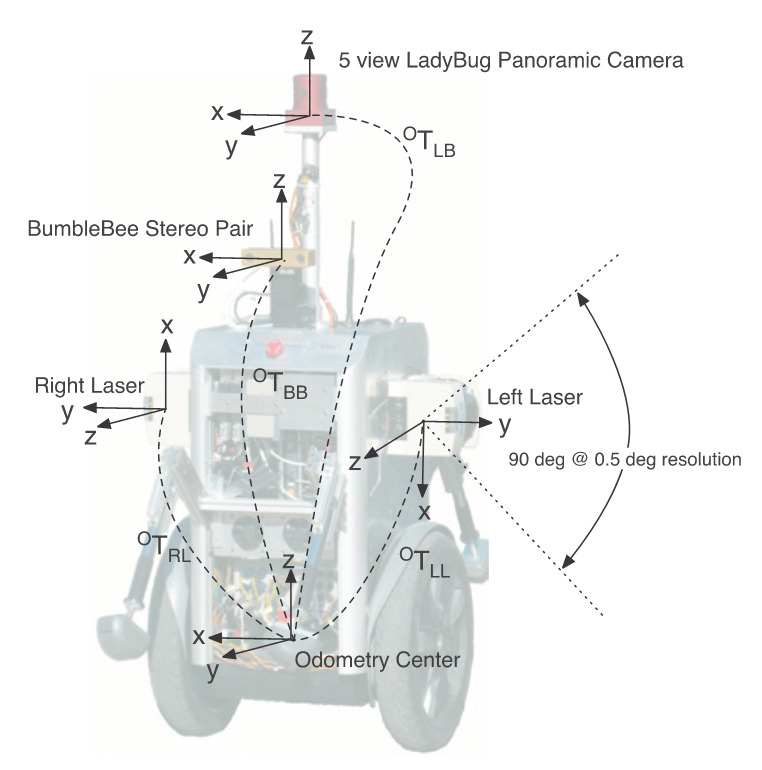
\includegraphics[height=0.3\linewidth]{assets/img/new-college.png}
	\hfill
	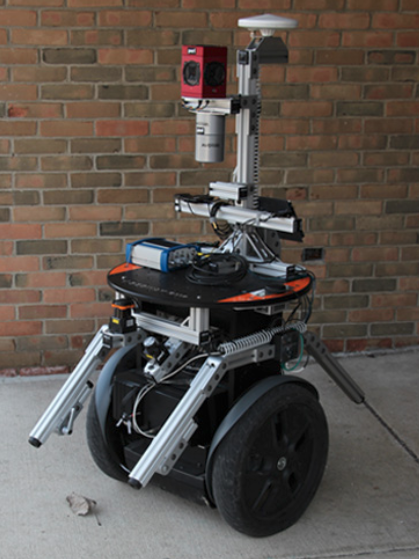
\includegraphics[height=0.3\linewidth]{assets/img/nclt.png}
	\hfill
	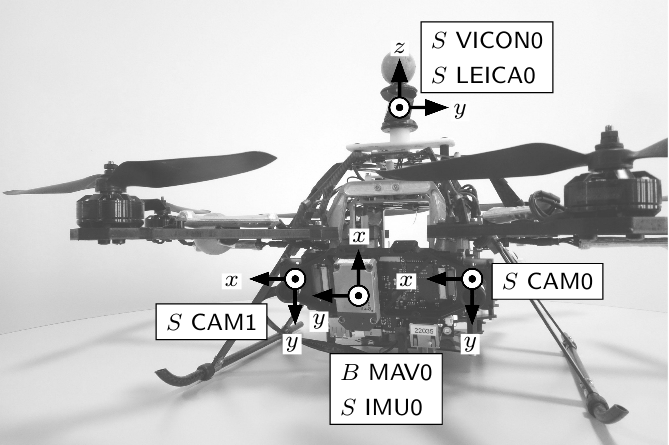
\includegraphics[height=0.3\linewidth]{assets/img/euroc-mav.png}
	\caption{Mobile robots used for SLAM datasets. From left to right,
	the Segway platform used in the New College dataset~\cite{smith2009new},
	the Segway platform used in the NCLT dataset~\cite{carlevaris2016university},
	the MAV used in the EuRoC MAV dataset~\cite{burri2016euroc}.}%
	\label{fig:mobile-robot-slam}
\end{figure}

A second wave of datasets,
represented in bold in Table~\ref{tab:vo-datasets},
has especially been targetting RGB-D cameras,
becoming popular after the launch of the Microsoft Kinect.
While the TUM RGB-D~\cite{sturm2012benchmark} and Bonn RGB-D~\cite{palazzolo2019iros}
datasets are recorded with real RGB-D sensors,
the ICL-NUIM~\cite{handa2014benchmark} dataset was generated (ray-traced rendered)
from synthetic 3D models of indoor scenes.
We are going to explain in more details the specificities of the TUM RGB-D and
ICL-NUIM datasets since these are the two we used to evaluate our direct RGB-D
visual odometry algorithm.

Finally, with the popularity of inertial sensors coupled with cameras in
modern smartphones enabling new augmented reality functionalities,
a regain in interest has been visible for 6 degrees of freedom visual inertial odometry (VIO).
While the EuRoC MAV~\cite{burri2016euroc} and TUM VI~\cite{schubert2018tum} datasets
are using high quality sensors,
the ADVIO dataset~\cite{cortes2018advio} is actually using regular smartphones sensors,
showing the importance of datasets with less precise data to improve algorithms robustness.
We provide a brief summary of these datasets properties in Table~\ref{tab:vo-datasets}.
Note that this is not an exhaustive list of available datasets but an overview
of the main ones for visual odometry.

\begin{table}[ht]
\centering
\resizebox{\textwidth}{!}{%
\begin{tabular}{llll}
Dataset
	& Year
    & Available data
	& Ground truth \\
    \midrule
New College~\cite{smith2009new}
	& 2009
	& \makecell[l]{GPS, IMU, wheel odometry,\\lidar, omnidirectional, stereo}
	& Dead-reckoned \\
\textbf{TUM RGB-D~\cite{sturm2012benchmark}}
	& 2012
	& IMU, \textbf{RGB-D}
	& Motion capture \\
KITTI~\cite{geiger2013vision}
	& 2013
	& GPS, IMU, lidar, stereo
	& High precision GPS/IMU \\
\textbf{ICL-NUIM~\cite{handa2014benchmark}}
	& 2014
	& \textbf{RGB-D}, 3D surface
	& Synthetic \\
NCLT~\cite{carlevaris2016university}
	& 2016
	& \makecell[l]{GPS, IMU, wheel odometry,\\lidar, omnidirectional}
	& RTK GPS and lidar SLAM \\
EuRoC MAV~\cite{burri2016euroc}
	& 2016
	& Stereo camera
	& Motion capture \\
TUM Mono~\cite{engel2016photometrically}
	& 2016
	& Mono camera
	& Closed loop \\
TUM VI~\cite{schubert2018tum}
	& 2018
	& IMU, Mono camera
	& Motion capture and closed loop \\
ADVIO~\cite{cortes2018advio}
	& 2018
	& Smartphone IMU and video
	& IMU with position fixes \\
\textbf{Bonn RGB-D~\cite{palazzolo2019iros}}
	& 2019
	& IMU, \textbf{RGB-D}, lidar
	& Motion capture \\
\end{tabular}%
} % end of resizebox
\caption{Visual odometry datasets}%
\label{tab:vo-datasets}
\end{table}


\subsubsection{Motion Capture for RGB-D Visual Odometry}%
\label{ssub:motion_capture}

The TUM RGB-D dataset~\cite{sturm2012benchmark} was the first
complete and rigorously detailed dataset for RGB-D visual odometry.
It is composed of 80 sequences, 47 for training with ground truth,
and 33 for validation only evaluated online, without ground truth.
The training sequences are arranged in six groups,
\begin{itemize}
\setlength\itemsep{-0.5em}
	\item testing and debugging (4 sequences), simple translation or rotation movements,
	\item handheld movements (11 sequences),
	\item robot movements (4 sequences),
	\item structure and texture (8 sequences), with difficult structure or texture patterns,
	\item dynamic objects (9 sequences),
	\item and object reconstruction (11 sequences).
\end{itemize}
As we can see, the dataset provides both easy sequences and sequences with
more difficult situations such as dynamic movements or poor textures
in the field of view of the camera.
It is thus a good benchmark of the robustness of visual odometry algorithms.
These sequences have been acquired by three different Kinect devices,
named fr1 (for ``Freiburg 1''), fr2 and fr3.
All their intrinsic parameters are available in the dataset.
The required robustness of the tested algorithms is also increased by the fact that
the color camera of the Kinect sensor has a rolling shutter.
We do not expect our algorithm to perform very well under those circumstances.

The ground truth camera poses are obtained thanks to an external motion capture system
based on MotionAnalysis~\cite{MotionAnalysis} hardware and software.
This setup is composed of eight 300 Hz Raptor-E high definition cameras,
equipped with infrared lights to illuminate passive markers attached to the Kinect.
After a detailed intrinsic and extrinsic parameters calibration of the system,
the authors estimate the relative position errors to be lower than 1 mm and 0.5 degrees.

\subsubsection{Synthetic Dataset Creation}%
\label{ssub:synthetic_dataset}

Most of the available visual odometry datasets lack a dense 3D surface ground truth
to be able to evaluate both the camera trajectory and the structure reconstruction.
To this end, Handa et al.\ created the ICL-NUIM dataset~\cite{handa2014benchmark}.
Contrary to most other datasets, the video sequences provided here are completely
generated by computer graphics, using the open-source ray tracing algorithm
POV-Ray~\cite{povray}.
The dataset is split into two rooms, a living room and an office,
and two scenarios, one noiseless and one with simulated noise.
The full pipeline is also provided as open source,
if one wishes to customize parts of it.
The geometry and some renders of the living room are displayed in Figure~\ref{fig:icl-nuim}.

\begin{figure}[t]
	\centering
	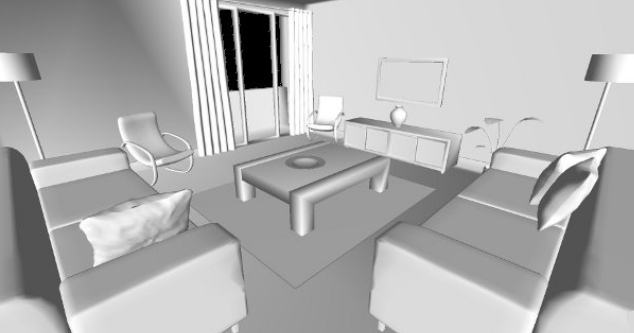
\includegraphics[height=0.3\linewidth]{assets/img/icl-nuim-geometry.png}
	\hfill
	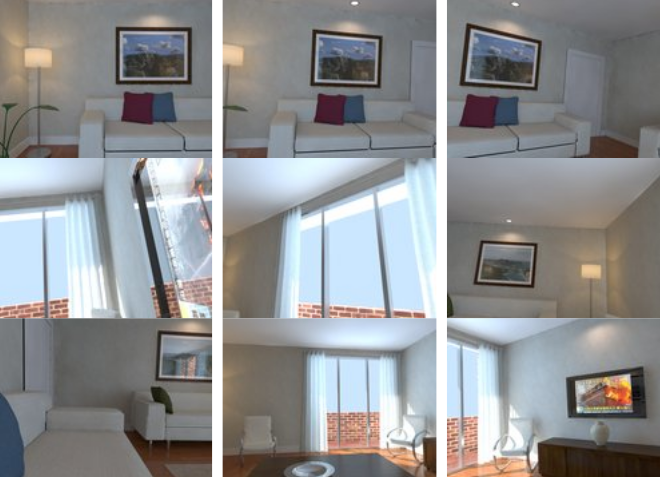
\includegraphics[height=0.3\linewidth]{assets/img/icl-nuim-povray.png}
	\caption{Geometry (left) and few rendered images (right)
	of the living room used for the ICL-NUIM dataset~\cite{handa2014benchmark}.}%
	\label{fig:icl-nuim}
\end{figure}

In order to test some visual odometry algorithms,
we are only going to use the eight noise-free sequences since realistic noisy sequences
are already evaluated with the TUM RGB-D dataset.
The trajectory ground truth generated by this ICL-NUIM dataset is thus error-free.
The color and depth images are also perfectly aligned,
timely synchronized and have no light exposure variations.
They still contain reflective surfaces and few other ligthing effects
not taken into account in our direct visual odometry modelization,
but the overall circumstances should be very favorable for our simple implementation.

\subsection{Evaluation Metrics}%
\label{sub:metrics}

There are basically two types of evaluation metrics,
those based on a ground truth, and those that are not.

\subsubsection{Metrics with Ground Truth, ATE and RPE}%
\label{ssub:metrics_gt}

The most straightforward method to evaluate a visual odometry trajectory
is to compare it with a reference trajectory, called ground truth.
This reference trajectory needs to be acquired with more precision
than the one being evaluated for the measure to make sense.
In our case, the TUM RGB-D dataset uses a motion capture system with sub-millimeter accuracy,
and the ICL-NUIM provides exact trajectories since it is a synthetic dataset.

The first evaluation metric commonly used is the absolute trajectory error (ATE).
We can consider the trajectory as a discrete set of camera poses
\[
	G_{\Omega} = \Set{g_{\tau}}{\tau \in \Omega,\ g_{\tau} \in SE(3)}
\]
where $\Omega$ is the set of discrete time events when camera poses are available.
In theory, the ATE can be computed as
\[
	\text{ATE} = \sum_{\Omega} d(g_{\tau}, \widehat{g}_{\tau})
\]
where $d(g_{\tau}, \widehat{g}_{\tau})$ can be thought of
as a distance between the estimated transformation $g_{\tau}$
and the ground truth transformation $\widehat{g}_{\tau}$.
Usually, we can consider two types of errors, the translation error
\[
	\| \text{trans}(\inv{\widehat{g}_{\tau}} \cdot g_{\tau}) \|
\]
and the rotation error
\[
	\measuredangle \, (\inv{\widehat{g}_{\tau}} \cdot g_{\tau})
\]
where $\measuredangle$ is the amplitude ($\geq 0$) of the rotation angle.
Since the rotation errors will also impact translation errors later,
it is common to only use the translation error when computing the ATE.
The two most widely used ATE metrics are the RMSE and the median scores
\[
	\text{ATE}_{\text{rmse}} =
		\left(
			% \frac{1}{\text{Card}(\Omega)} \sum_{\Omega}
			\mean
			{\| \text{trans}(\inv{\widehat{g}_{\tau}} \cdot g_{\tau}) \|^2}
		\right)^{1/2}
	\quad \text{and} \quad
	\text{ATE}_{\text{median}} =
		\text{median} \left( \| \text{trans}(\inv{\widehat{g}_{\tau}} \cdot g_{\tau}) \| \right).
\]
The median is a better indicator of the algorithm precision,
while the RMSE better reflects the presence (or absence) of outliers,
i.e.\ the global robustness of the algorithm.

In practice, we should note that the ground truth and estimated trajectory
are not expressed in the same reference frame.
It is thus necessary to first align the two trajectories.
This is usally done with a principal component analysis (PCA)
of the trajectories.
It is also important to note that the ground truth and estimated trajectories
are not sampled at the same timings and frequency.
Therefore, it is also necessary to correctly associate poses of each trajectory,
which is reasonably easy when timestamps have been synchronized in the dataset.
One of the main issues of the ATE is that drifts have higher impact at the beginning
of the sequence than at the end.
To better evaluate long sequences we thus use another metric,
the relative pose error (RPE).

Contrary to the ATE, which evaluates absolute errors on associated pairs of poses,
the RPE compares the relative motion in a sliding window along the sequence.
The size of the window is usually a fixed travelled distance or time interval.
We will detail for example the computation of the RPE at 1 second.
For each associated pair of estimated and ground truth poses $(g_{\tau}, \widehat{g}_{\tau})$,
we consider another pair $(g_{\tau'}, \widehat{g}_{\tau'})$
delayed by 1 second ($\tau' \approx \tau + 1s$).
The camera motion between $\tau$ and $\tau'$ in the estimated trajectory is
$\Delta_{\tau \tau'} g = \inv{g_{\tau}} \cdot g_{\tau'}$
and the camera motion in the ground truth trajectory is
$\Delta_{\tau \tau'} \widehat{g} = \inv{\widehat{g}_{\tau}} \cdot \widehat{g}_{\tau'}$.
The relative pose error is thus computed as
\[
	\text{RPE} = \sum_{\Omega'} d(\Delta_{\tau \tau'} g, \Delta_{\tau \tau'} \widehat{g})
\]
where $d(\cdot, \cdot)$ is similar than for the ATE,
and $\Omega'$ is the set of regularly spaced pairs,
whether it is a duration, like 1 second, or a distance like 1 meter.

\alert{Ajouter un schéma RPE avec les notations précédentes.}


\subsubsection{Metrics without Ground Truth}%
\label{ssub:metrics_no_gt}

In some conditions, such as long handheld outdoor trajectories,
retrieving a ground truth might be problematic.
Yet it is still possible to partially evaluate the precision of an algorithm,
or rather its robustness to drifts and losses.
Indeed, in absence of a full sequence ground truth,
it is still possible to evaluate the tracking of loops.
It is important to note that global loop closure detections must
be deactivated in the algorithms for these measures to make sense.

One method consists in computing loop closure and pose graph optimization
and then compare the trajectory before and after.
If the drifts of the tracking are not too extreme and do not prevent the pose graph optimization,
this error can be representative of the visual odometry performance.

Another approach consists in specifically designing the dataset sequences
to start and end at the same location, such that both ends of the trajectory
can be precisely aligned.
This is the approach taken in~\cite{engel2016photometrically}.
The error computed is then the accumulated drift between the sequence when aligned
to the start and when aligned to the end of the partial ground truth trajectory.


\subsection{Setup and Algorithms Evaluation}%
\label{sub:algorithms_eval}

In this section, we describe how we evaluated our VORS implementation
and compared it to other open source C++ algorithms.
We focused on RGB-D visual odometry, and therefore used
both the TUM RGB-D~\cite{sturm2012benchmark} and ICL-NUIM~\cite{handa2014benchmark} datasets.

\subsubsection{The TUM RGB-D Dataset Format}%
\label{ssub:dataset-format}

The TUM RGB-D dataset is well specified and as a result,
others including ICL-NUIM follow the same format.
We therefore also base our evaluation setup on the TUM RGB-D format.
The general structure of such dataset is as follows.
\lstinputlisting[%
  language=bash,
  caption={General structure of the TUM RGB-D dataset format.},
  label={lst:dataset}
]{assets/code/dataset.txt}
The files \verb|rgb.txt| and \verb|depth.txt| list all images with their associated timestamps.
The RGB-D visual odometry algorithms also need the correspondences between color
and depth images, so if not present, the first step is usually to run
a provided \verb|associate.py| script to generate an \verb|associations.txt| file
from the \verb|rgb.txt| and \verb|depth.txt| files.
Each line of that file contains a pair of RGB and depth images with their respective timestamps.
Color images are stored as 640x480 8-bit RGB images in the PNG format.
Depth images are stored as 640x480 16-bit monochrome images in the PNG format.
Depth images are scaled by a factor of 5000, i.e.\ a pixel value of 5000 corresponds
to a distance of 1 meter.
Theoretically depth images thus have a precision of 0.2 mm for a range of
0 to roughly 13~meters.
The ground truth trajectory is provided in the \verb|groundtruth.txt| file as follows.
\lstinputlisting[%
  language=bash,
  caption={Ground truth trajectory format.},
  label={lst:groundtruth}
]{assets/code/groundtruth.txt}
The timestamp is the POSIX time of the given pose,
i.e.\ the number of seconds elapsed since 1970, January 1st.
The coefficients \verb|tx|, \verb|ty|, \verb|tz|, are the coordinates
of the optical center of the color camera with respect to a given world frame.
The coefficients \verb|qx|, \verb|qy|, \verb|qz|, \verb|qw| are the parameters of the quaternion
describing the orientation of the color camera.
The last coefficient \verb|qw| is the real part of the quaternion.

\subsubsection{Open Source Algorithms and Provided Setup}%
\label{ssub:algorithms_and_setup}

In addition to VORS, we evaluated five other open source algorithms for RGB-D visual odometry,
namely DVO~\cite{kerl2013robust}, Fovis~\cite{huang2017visual},
and three variants of the OpenCV RGB-D odometry module
based on~\cite{newcombe2011kinectfusion, steinbrucker2011real}.
For each one of those six algorithms, we implemented a small program
performing the following operations (pseudo code).
\lstinputlisting[%
  language=bash,
  caption={Outline of the common RGB-D odometry program implemented for every tested algorithm.},
  label={lst:track}
]{assets/code/track.txt}
All those algorithms except VORS are C++ programs with different complexity of build,
due to dependency issues.
DVO for example would not compile anymore with recent versions of
the Sophus~\cite{sophus} library for Lie algebra
due to missing re-orthogonalization of the rotation matrix after optimization increments.
Therefore, we are providing clear installation instructions as well as
a Docker container ready for compilation of all 6 programs.
This setup is open sourced under GPL license
at \url{https://github.com/mpizenberg/rgbd-tracking-evaluation}.

\subsubsection{Evaluation Results}%
\label{ssub:eval_results}

We evaluated all algorithms both on the ICL-NUIM dataset and on the TUM RGB-D dataset,
constituting a total of 55 sequences.
As visible in Figure~\ref{fig:rpe_median_all},
our implementation (VORS) performs similarly than DVO, Fovis and OCV-RGBD.
It is coherent since these four algorithms use both the visual information of the color image
and the depth map to estimate the camera motion.
OCV-ICP however, which only uses the depth map,
is unable to track the camera movements in the majority of sequences.
The OCV-RGBD-ICP variant, which is a mixed approach minimizing both energies
of OCV-RGBD and OCV-ICP, inherits from the same tracking difficulties as OCV-ICP.\@

\begin{figure}[ht]
	\centering
	\begin{tikzpicture}
    \begin{axis}
    [
    ytick={1,2,3,4,5,6,7}
    , yticklabels={vors,fovis,dvo,ocv-rgbd,ocv-rgbd-icp,ocv-icp,still},
    ]

        \addplot+[
        color=black,
        style=solid,
        boxplot prepared={
            median=0.022110,
            upper quartile=0.049158,
            lower quartile=0.009474,
            upper whisker=0.353370,
            lower whisker=0.000536
        },
        ] coordinates {};
        \addplot+[
        color=black,
        style=solid,
        boxplot prepared={
            median=0.034459,
            upper quartile=0.061213,
            lower quartile=0.011091,
            upper whisker=0.277995,
            lower whisker=0.002489
        },
        ] coordinates {};
        \addplot+[
        color=black,
        style=solid,
        boxplot prepared={
            median=0.026247,
            upper quartile=0.061083,
            lower quartile=0.016640,
            upper whisker=0.223077,
            lower whisker=0.001971
        },
        ] coordinates {};
        \addplot+[
        color=black,
        style=solid,
        boxplot prepared={
            median=0.030116,
            upper quartile=0.072295,
            lower quartile=0.013935,
            upper whisker=0.300951,
            lower whisker=0.001996
        },
        ] coordinates {};
        \addplot+[
        color=black,
        style=solid,
        boxplot prepared={
            median=0.186426,
            upper quartile=0.260719,
            lower quartile=0.059544,
            upper whisker=0.439046,
            lower whisker=0.000050
        },
        ] coordinates {};
        \addplot+[
        color=black,
        style=solid,
        boxplot prepared={
            median=0.186426,
            upper quartile=0.260719,
            lower quartile=0.059544,
            upper whisker=0.439046,
            lower whisker=0.000033
        },
        ] coordinates {};
        \addplot+[
        color=black,
        style=solid,
        boxplot prepared={
            median=0.186514,
            upper quartile=0.261502,
            lower quartile=0.059499,
            upper whisker=0.439919,
            lower whisker=0.002305
        },
        ] coordinates {};    \end{axis}
\end{tikzpicture}

	\caption{Distribution of the median relative pose error (RPE) at 1 second on all 55 sequences,
	composed of 47 TUM sequences and 8 ICL-NUIM sequences.}%
	\label{fig:rpe_median_all}
\end{figure}

Out of 55 sequences taken into account in the Figure~\ref{fig:rpe_median_all},
the wide majority (47) comes from the TUM RGB-D dataset.
VORS, which does not implement robust approaches,
should perform better for the synthetic sequences of the ICL-NUIM dataset than
for the real sequences of the TUM dataset.
Figure~\ref{fig:rpe_median_icl} thus presents the same plot than
Figure~\ref{fig:rpe_median_all} but restricted to the 8 ICL-NUIM sequences.
As we can see, VORS is performing remarkably in these conditions.
Other noteworthy details are exacerbated by this plot.
Both geometric odometries (OCV-ICP and OCV-RGBD-ICP) perform extremely well
thanks to the high precision dense depth maps provided by the dataset.
One should note that this precision comes at the price of time.
The first ICL sequence for example takes three times longer
with OCV-ICP than with Fovis, VORS and DVO, all comparable in speed.
It is also notable that Fovis is having more issues tracking those sequences.
It can be explained by the nature of this algorithm, which is indirect,
based on FAST features, contrary to VORS, DVO and OCV-RGBD which are
direct visual odometry algorithms.
The synthetic nature of the images, and lack of unique textures compared
to real images is degrading the detection rate of Fovis FAST descriptors.

\begin{figure}[ht]
	\centering
	\begin{tikzpicture}
    \begin{axis}
    [
    ytick={1,2,3,4,5,6,7}
,    yticklabels={vors,fovis,dvo,ocv-rgbd,ocv-rgbd-icp,ocv-icp,still},
    ]

        \addplot+[
        color=black,
        style=solid,
        boxplot prepared={
            median=0.000651,
            upper quartile=0.000693,
            lower quartile=0.000605,
            upper whisker=0.000794,
            lower whisker=0.000536
        },
        ] coordinates {};
        \addplot+[
        color=black,
        style=solid,
        boxplot prepared={
            median=0.007218,
            upper quartile=0.009637,
            lower quartile=0.004787,
            upper whisker=0.010963,
            lower whisker=0.002489
        },
        ] coordinates {};
        \addplot+[
        color=black,
        style=solid,
        boxplot prepared={
            median=0.002200,
            upper quartile=0.002373,
            lower quartile=0.002093,
            upper whisker=0.004196,
            lower whisker=0.001971
        },
        ] coordinates {};
        \addplot+[
        color=black,
        style=solid,
        boxplot prepared={
            median=0.002500,
            upper quartile=0.002685,
            lower quartile=0.002360,
            upper whisker=0.003010,
            lower whisker=0.001996
        },
        ] coordinates {};
        \addplot+[
        color=black,
        style=solid,
        boxplot prepared={
            median=0.000086,
            upper quartile=0.000092,
            lower quartile=0.000080,
            upper whisker=0.000107,
            lower whisker=0.000050
        },
        ] coordinates {};
        \addplot+[
        color=black,
        style=solid,
        boxplot prepared={
            median=0.000053,
            upper quartile=0.000054,
            lower quartile=0.000048,
            upper whisker=0.000057,
            lower whisker=0.000033
        },
        ] coordinates {};
        \addplot+[
        color=black,
        style=solid,
        boxplot prepared={
            median=0.007036,
            upper quartile=0.009313,
            lower quartile=0.003299,
            upper whisker=0.010179,
            lower whisker=0.002305
        },
        ] coordinates {};    \end{axis}
\end{tikzpicture}

	\caption{Distribution of the median relative pose error (RPE) at 1 second
	on the 8 ICL-NUIM sequences.}%
	\label{fig:rpe_median_icl}
\end{figure}

Instead of using the median RPE,
which pictures the overall precision of the algorithms,
Figure~\ref{fig:rpe_rmse_icl} represents the RMSE RPE,
which better reflects the robustness to outliers.
As visible in that figure, VORS has a long tail of highly
erroneous motion tracking.
High RMSE errors are better understood when looking at the
detailed RPE of one sequence, as shown in Figure~\ref{fig:rpe_icl3}.
In the end, even though our visual odometry implementation in Rust (VORS)
has robustness issues due to previously discussed challenges,
we provide a precise, state of the art RGB-D visual odometry,
easy to compile, to use and as we will develop next,
easy to port to WebAssembly.
VORS thus enables the exploration of efficient interactive
visual odometry on the Web, which we finally present next.

\alert{Parler plus de la dernière figure.
Ajouter une discussion un peu plus fournie
sur les perfs de VORS en bilan.
En transition mentionner que on va pouvour corriger certains
défauts de manière interactive.}

\begin{figure}[ht]
	\centering
	\begin{tikzpicture}
    \begin{axis}
    [
    ytick={1,2,3,4,5}
,    yticklabels={vors,dvo,ocv-rgbd,ocv-rgbd-icp,ocv-icp},
    ]

        \addplot+[
        color=black,
        style=solid,
        boxplot prepared={
            median=0.002240,
            upper quartile=0.011160,
            lower quartile=0.001571,
            upper whisker=0.015429,
            lower whisker=0.000991
        },
        ] coordinates {};
        \addplot+[
        color=black,
        style=solid,
        boxplot prepared={
            median=0.004430,
            upper quartile=0.005419,
            lower quartile=0.003908,
            upper whisker=0.007656,
            lower whisker=0.003717
        },
        ] coordinates {};
        \addplot+[
        color=black,
        style=solid,
        boxplot prepared={
            median=0.006143,
            upper quartile=0.008625,
            lower quartile=0.004346,
            upper whisker=0.009195,
            lower whisker=0.003350
        },
        ] coordinates {};
        \addplot+[
        color=black,
        style=solid,
        boxplot prepared={
            median=0.000223,
            upper quartile=0.000917,
            lower quartile=0.000203,
            upper whisker=0.005320,
            lower whisker=0.000154
        },
        ] coordinates {};
        \addplot+[
        color=black,
        style=solid,
        boxplot prepared={
            median=0.000817,
            upper quartile=0.006016,
            lower quartile=0.000191,
            upper whisker=0.008085,
            lower whisker=0.000113
        },
        ] coordinates {};    \end{axis}
\end{tikzpicture}

	\caption{Distribution of the RMSE relative pose error (RPE) at 1 second
	on the 8 ICL-NUIM sequences.}%
	\label{fig:rpe_rmse_icl}
\end{figure}

\begin{figure}[ht]
	\centering
	\begin{tikzpicture}
\begin{axis}[
		xlabel=Frame,
		ylabel=RPE,
		ymax=0.05
	]
	\addplot[color=blue] table [x=timestamp,y=t_err_s,col sep=comma]{assets/csv/rpe_1s_still.csv};
	\addlegendentry {still}
	\addplot[color=green] table [x=timestamp,y=t_err_s,col sep=comma]{assets/csv/rpe_1s_dvo.csv};
	\addlegendentry {dvo}
	\addplot[color=red] table [x=timestamp,y=t_err_s,col sep=comma]{assets/csv/rpe_1s_vors.csv};
	\addlegendentry {vors}
\end{axis}
\end{tikzpicture}

	\caption{Relative pose error (RPE) at 1 second for the third
	living room sequence of the ICL-NUIM dataset.}%
	\label{fig:rpe_icl3}
\end{figure}

\clearpage
\section{Interactive VORS on the Web}%
\label{sec:interactive-vors}

We previously quantitatively validated VORS viability for the visual odometry task.
In this final section we detail how it can be usable directly on the Web.
We also attempt at showcasing the potential of such exposure with
an example use case of manual human intervention to detect and rectify drifts.

\subsection{Port of VORS to WebAssembly}%
\label{sub:vors-port-wasm}

\subsubsection{VORS in WebAssembly}%

Except from two little hurdles that we are going to detail,
the port of VORS to WebAssembly was straightforward,
as expected for a Rust-only project.
VORS code base is organized as a library providing a rich API,
accompanied by a small binary program performing the actual visual odometry
on a dataset provided as a command line argument.
Porting VORS is thus a matter of two tasks,
(1) being able to compile the library to the WebAssembly target,
(2) rewrite a small WebAssembly program replacing the command line program
in the context of a Web browser.
The first task is immediately validated by running
\verb|cargo build --target wasm32-unknown-unknown|,
confirming the ability to compile VORS to WebAssembly.
The second task requires more work,
due to the different natures of native command line applications and Web browsers.

\subsubsection{Loading Data as a Tar Archive}%

Native programs have the ability to interact with the underlying operating system.
Web applications however are sandboxed, for security reasons reminded
in Chapter~\ref{cha:performant_web_applications} on performant Web applications.
The seemingly simple task of loading images for the dataset directory
thus becomes impossible.
The simplest alternative, which is the one we chose,
consists in loading a \verb|tar| archive of the entire dataset through
the file upload mechanism, making the archive content available in the browser memory.
This has two constraints, one on memory the other on the application program.

Current Web APIs prevent us from loading the archive directly on the WebAssembly memory.
As a consequence, the archive is loaded inside the application JavaScript memory,
and we then duplicate it in the WebAssembly module memory.
For an unknown period of time, until the browser decides to release the JavaScript buffer,
the application will consume a memory of double the archive size.
The full first sequence of the ICL-NUIM dataset for example weighs 800 MB,
resulting in 1.6 GB of allocated memory by the application in the browser.

The other change has to occur in the program code, now reading files from an archive
instead of from the file system.
For this task, we used the \verb|tar-rs| library~\cite{tar-rs},
which brought the first hurdle by not compiling to WebAssembly
due to the presence of OS-specific code for file time management.
Fortunately, simply adding compiler guards in that library to deactivate
the incriminating functions from the public API when compiling to WebAssembly was sufficient.

\subsubsection{PNG Image Reading}%

The next technical challenge was a performance one.
We managed to get VORS compiling and running as a WebAssembly module,
but the performances dropped drastically, from 30 frames per second (fps)
in the native case to less than 10 fps in WebAssembly.
After some performance analysis, we identified the culprit as
the PNG image decoding of frames.
Figure~\ref{fig:png-perf} spotlights that the majority of the time
is spent in decoding both images instead of in the visual odometry algorithm.

\begin{figure}[ht]
	\centering
	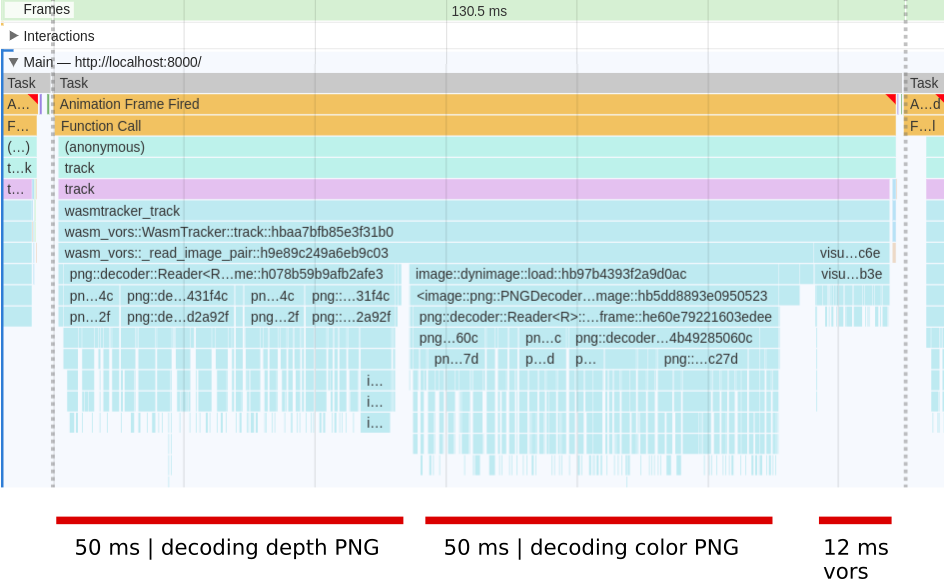
\includegraphics[width=\linewidth]{assets/img/png-perf-profile-annotated.png}
	\caption{Flame graph of VORS WebAssembly performances with the PNG Rust crate.
	The majority of the time is spent decoding RGB-D images.}%
	\label{fig:png-perf}
\end{figure}

From the fact that OpenCV decodes images much faster,
and that Rust should have similar performances than C++,
we decided to give a try at a new PNG decoder.
Our implementation keeps in mind that it should be ``Wasm-friendly'',
meaning we limit the amount of memory allocations,
which are more costly in WebAssembly.

The PNG specification is available online.
Under the hood, the data is compressed with the deflate algorithm,
whose specification is also available online.
PNG is a simple structured format.
A file contains successive data blocks called chunks of different types.
The most interesting types are IHDR (header), IDAT (data) and IEND (end of file).
The body of the image is composed by successive IDAT blocks
containing transformed lines of the image (called ``filtered'') to reduce entropy,
then compressed with the deflate algorithm.
We have implemented the parsing with a fast parser combinator library,
and the unfiltering is rather simple.
We did not reimplement the inflate algorithm
since there are already high performance Rust-only libraries for this task.
After a few round of optimizations,
we managed to get great decoding performances,
especially in WebAssembly compared to the library we used initially.
Table~\ref{tab:png-perf} summarizes performances on few images we used locally
and clearly shows the improvement from the default Rust PNG library.
OpenCV performances are included for comparison.
As a result, we managed to get VORS compiling and running at similar speed in the browser.

\begin{table}[ht]
\centering
% \resizebox{\textwidth}{!}{%
\begin{tabular}{llllll}
Image & us & png crate & OpenCV & us (wasm) & png (wasm) \\
    \midrule
depth.png & 4.0 ms & 9.1 ms & 4.0 ms & 5.5 ms & 30.7 ms \\
rgb.png & 6.6 ms & 16.0 ms & 6.5 ms & 13.7 ms & 52.1 ms \\
\end{tabular}%
% } % end of resizebox
\caption{Decoding performances of our PNG decoder.}%
\label{tab:png-perf}
\end{table}

\subsection{Interactive VORS Web Interface}%
\label{sub:vors-web}

\subsubsection{Overview of the Interface}%

Interactive VORS Web interface is visible in Figure~\ref{fig:interactive-vors-interface}
and is composed of three parts,
\begin{itemize}
\setlength\itemsep{-0.5em}
	\item the control bar at the bottom, with a timeline and some buttons,
	\item the point cloud 3D visualization in the center,
	\item and the image thumbnail of the current keyframe on the left.
\end{itemize}
Contrary to structure from motion where images are not guaranted to be in any specific order,
visual odometry has the advantage of dealing with video data.
The timeline thus enables movement along the temporal axis.
It is a one-dimensional control that is well known thanks to its pervasive usage for videos.
The frames accessible from the timeline are restricted to the keyframes of the visual odometry.
As explained in Section~\ref{sub:multi-res-direct-image-alignment},
they are the frames used as reference for the direct image alignment.
A thumbnail of the current keyframe is located at the top left corner of the Web interface.
For each keyframe, we use the depth information of the sparse candidate points
to retrieve their 3D coordinates.
The number of candidate points is variable but in the order of a thousand
to ten thousands points per keyframe.
Those 3D points are stored in an array buffer,
then used for a point cloud visualization,
located at the center of the interface.
The sparse candidate points corresponding to the current keyframe
are visualized in red, to ease the mental association between the keyframe thumbnail
and the corresponding location in the complete point cloud.
The reader may notice in Figure~\ref{fig:interactive-vors-interface}
that the point cloud and the keyframe thumbnail are mirrored.
This is due to the ray tracer employed in the ICL-NUIM dataset,
which uses a left-handed coordinate system.

\begin{figure}[ht]
	\centering
	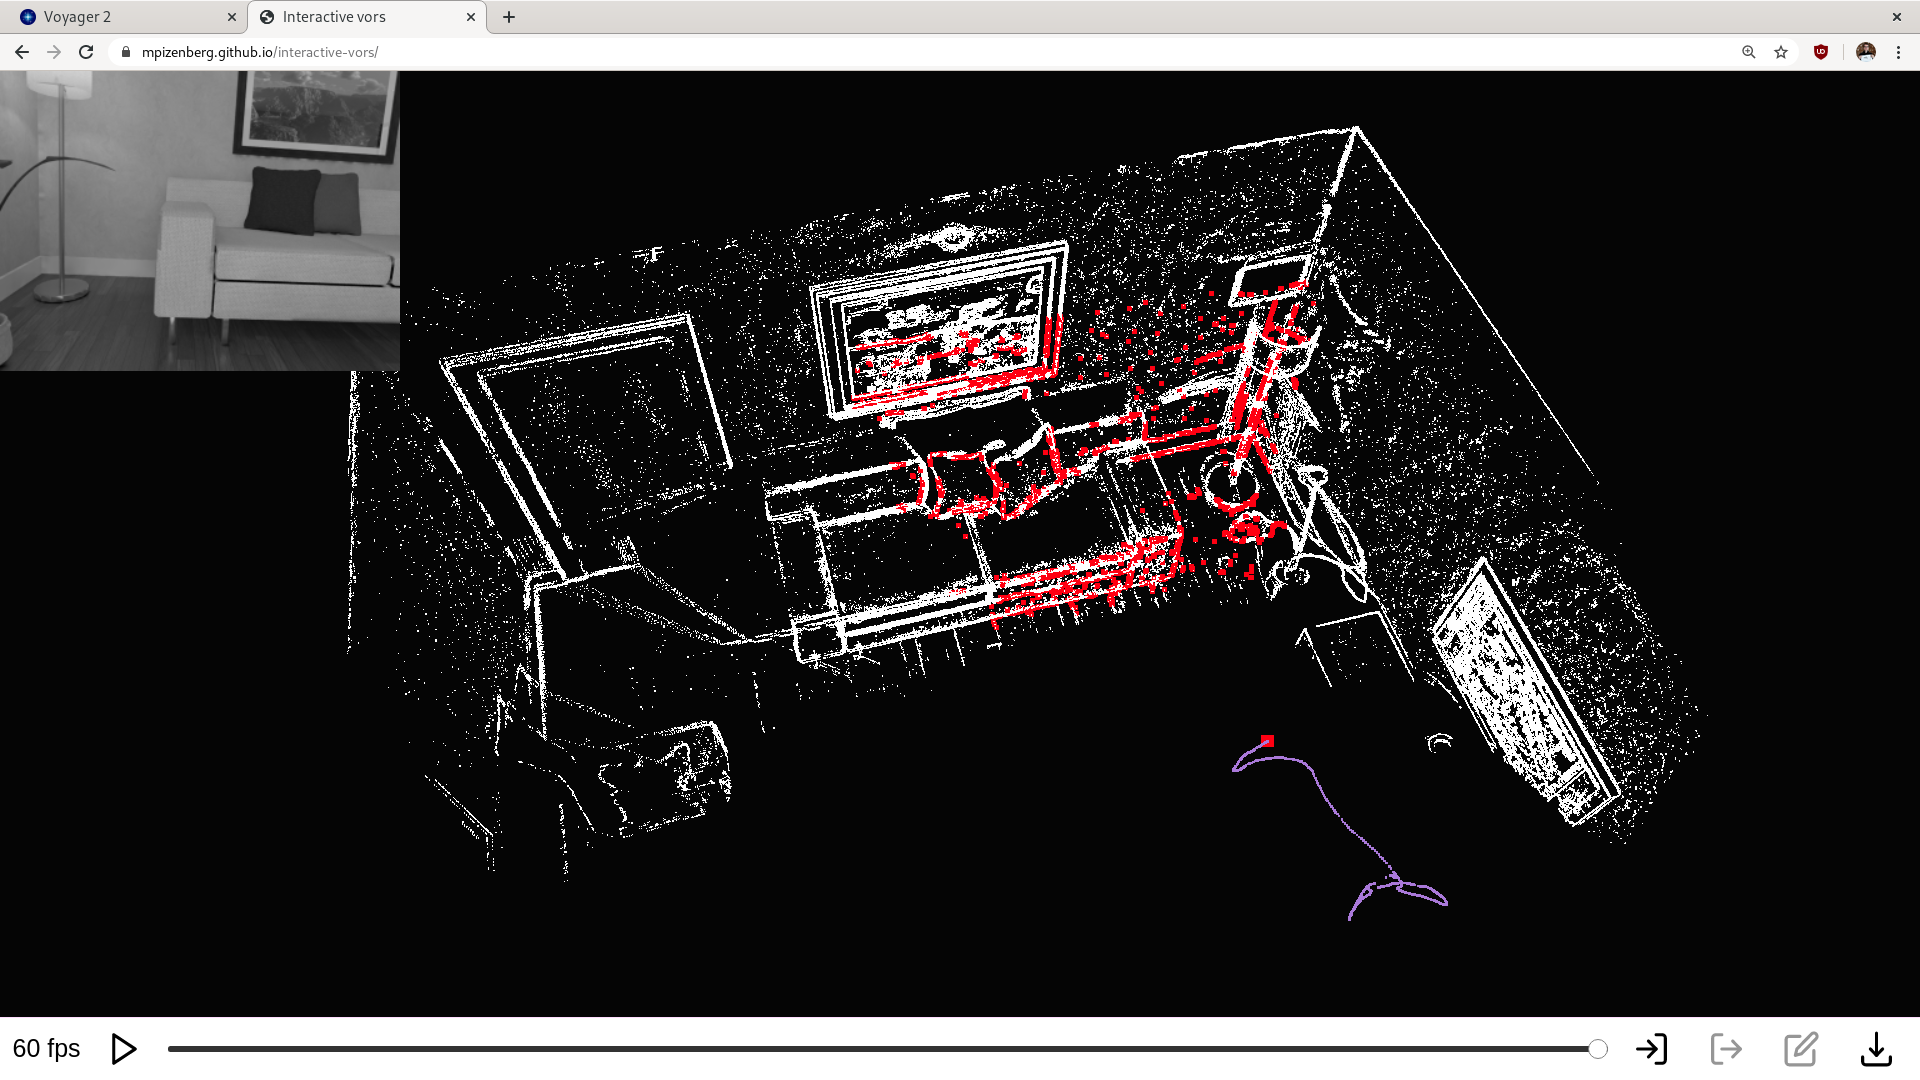
\includegraphics[width=\linewidth]{assets/img/interactive-vors.png}
	\caption{Interactive VORS Web Interface.}%
	\label{fig:interactive-vors-interface}
\end{figure}

\subsubsection{Visualization Challenges}%

Is Rust mature enough to write the visualization code in Rust native,
and compile it to WebAssembly?
Even though the field is exciting and buzzing, the short answer is no.
The Rust ecosystem is still lacking in the domain of graphical user interfaces (GUI).
As of 2019, only a handful of libraries enable 3D graphics,
often as bindings to other C++ libraries.

Currently, the four main APIs for graphics are OpenGL, Vulkan, DirectX and Metal.
OpenGL is an open standard developed by the Khronos group since 1992.
It is easy and high level, but becoming obselete
when efficient use of current graphics card hardware is needed.
DirectX is Microsoft alternative to OpenGL.\@
Up until DirectX 11, it was also a high level API,
but starting from DirectX 12, became lower level and more efficient.
Vulkan and Metal are also part of this renewal of graphics APIs
targetting more efficient usage of the hardware architecture.
Vulkan is open and developed by Khronos while Metal is Apple property.

Just as WebGL was introduced as a Web version of OpenGL,
a new standard is rising from the Vulkan API, called WebGPU.\@
Unfortunately, as of August 2019, WebGPU is only supported on Chrome canary for OSX.\@
The only viable option for our visualization is thus the duo OpenGL/WebGL.\@
After trying few Rust libraries, the conclusion is that currently,
the only way of reaching decent performances with WebGL for large point clouds,
is directly with a WebGL framework,
not with automatic conversion from a Rust native OpenGL code.
As a consequence, our point cloud visualization is based on ThreeJS~\cite{threejs},
a JavaScript 3D library.
The points buffers used for the visualizations are efficiently referenced
directly from the WebAssembly memory.
This mutable memory manipulation has been challenging and error-prone
but we eventually managed to get the visualizations working correctly.

\subsection{Human in the Loop Closure}%
\label{sub:human-loop-closure}

As discussed in Section~\ref{sub:algorithms_eval},
VORS is a precise visual odometry algorithm, prone to big local drifts.
The resulting point cloud visualizations contain parts that seem to be duplicated,
as in Figure~\ref{fig:interactive-vors-drift}.
This kind of observations is common in the presence of loops in the sequence.
In a SLAM context, presented in Section~\ref{sub:relation-visual-slam},
this type of drifts may be corrected by loop closure detection and pose graph optimization.
In this section however, we put the human in the loop, instead of automatic loop closure.

\begin{figure}[ht]
	\centering
	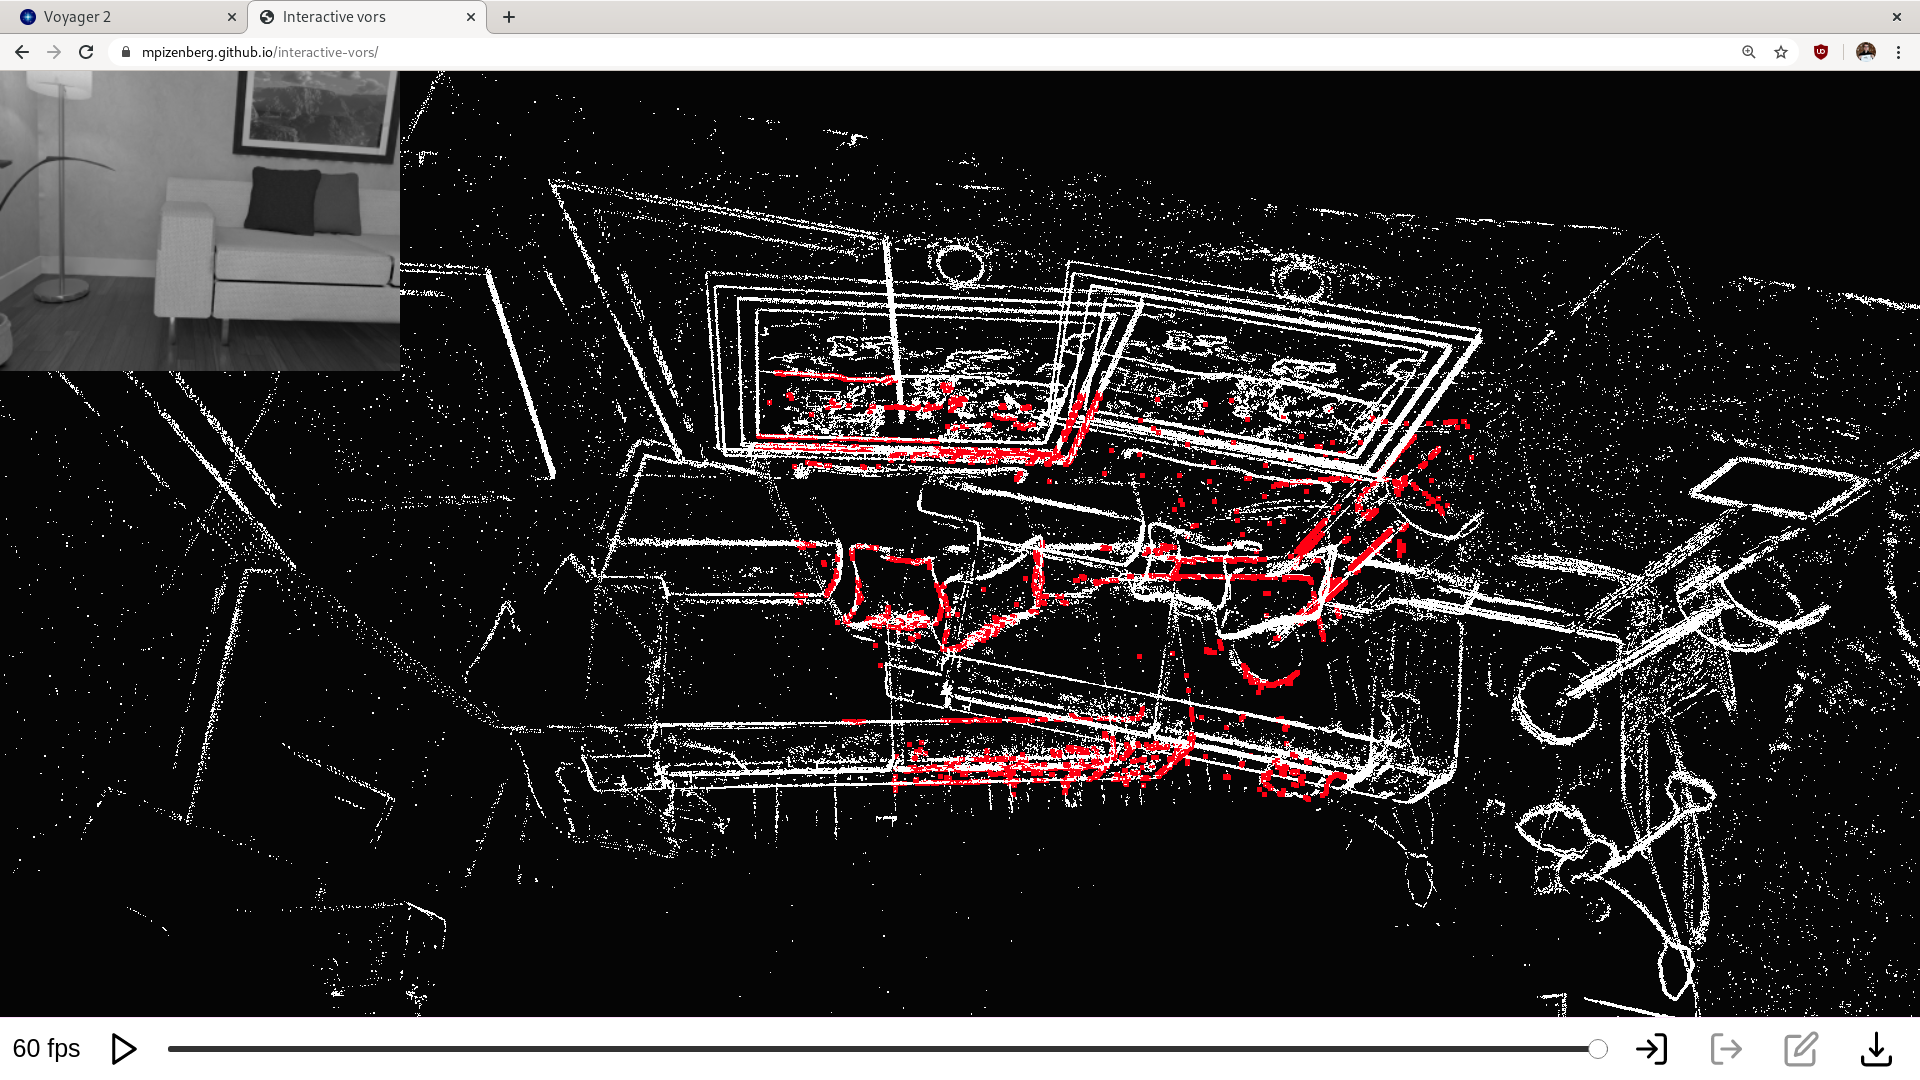
\includegraphics[width=\linewidth]{assets/img/interactive-vors-drift.png}
	\caption{Duplication of the point cloud due to drifts.}%
	\label{fig:interactive-vors-drift}
\end{figure}

\subsubsection{Automatic Registration}%

In traditional indirect SLAM algorithms, points of interests are retrieved for all keyframes
and their descriptors are classified with techniques such as ``bag of words''.
Then typical indexing and search algorithms are applied to identify similar keyframes.
In our case, the identification is performed by a human interaction,
clicking on the buttons in the toolbar for the reference keyframe
and the one that need re-ajusting.
Once two keyframes are selected, the next step consists in computing
the camera motion between those.

Usually, one would match all keypoints in the pair of images
and use a robust version of the 8-point algorithm if there is no depth information,
or a robust PNP algorithm if depth information is known.
We thus tried to perform keypoints detection and matching for the pair of keyframes.
There exist many keypoint descriptors for this task.
Some well known are ORB, SIFT, FAST and A-KAZE,
with a Rust implementation of A-KAZE features already available.
Unfortunately, due to the low textured images of the synthetic dataset,
the number of matches for selected pairs of keyframes are in the order of 20,
with multiple wrong matches, leading to unreliable camera motion.
It is the same issue that the one degrading Fovis performances in the ICL-NUIM dataset.

The second approach consists in computing direct image alignment from the reference frame.
Unfortunately, the keyframes matched by the user are not always similar enough
for the direct image alignment to converge to the correct motion.
This leads us to another manual human intervention.

\subsubsection{Manual P3P Intervention}%

As presented in Section~\ref{sub:feature-based} on feature-based motion estimation,
P3P is a minimal PnP (``perspective-n-points'') solver.
It enables motion estimation from a set of three points with depth information
in the reference frame and three associated points in the other frame.
We therefore use the keyframe thumbnails for an annotator to click on three
corresponding points, as visualized in Figure~\ref{fig:p3p}.

\begin{figure}[ht]
	\centering
	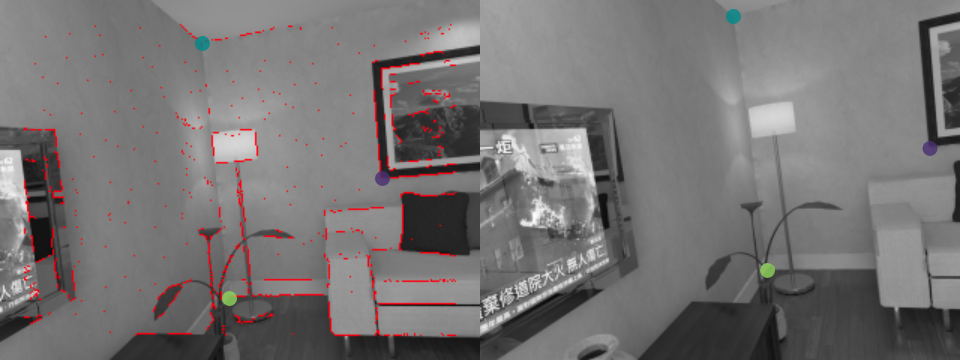
\includegraphics[width=\linewidth]{assets/img/p3p.png}
	\caption{Clicking interaction on keyframes thumbnails to perform P3P.}%
	\label{fig:p3p}
\end{figure}

The P3P algorithm may return 0 to 4 potential solutions.
Usually, those are disambiguated by looking at additional associated points.
In our case, we decided to let the human user pick the correct option.
Each potential solution is displayed with a different color.
The photometric reprojection error of the lowest image resolutions of the pyramid
is computed to estimate the probability of each camera position,
displayed in the lower right corner of the interface.
The user has to click on the correct option to validate it.
Figure~\ref{fig:p3p-two-poses} depicts an example situation where two potential
P3P poses are proposed in addition to a misaligned initial proposition in red.
Once a new camera pose is chosen for the second keyframe,
the visual odometry may be restarted for all subsequent frames.
Our Rust implementation of P3P is based on Persson and Nordberg's solver~\cite{persson2018lambda}
and published as an open source library under the Rust Computer Vision (rust-cv)
Github organization~\cite{rust-p3p}.

\begin{figure}[t]
	\centering
	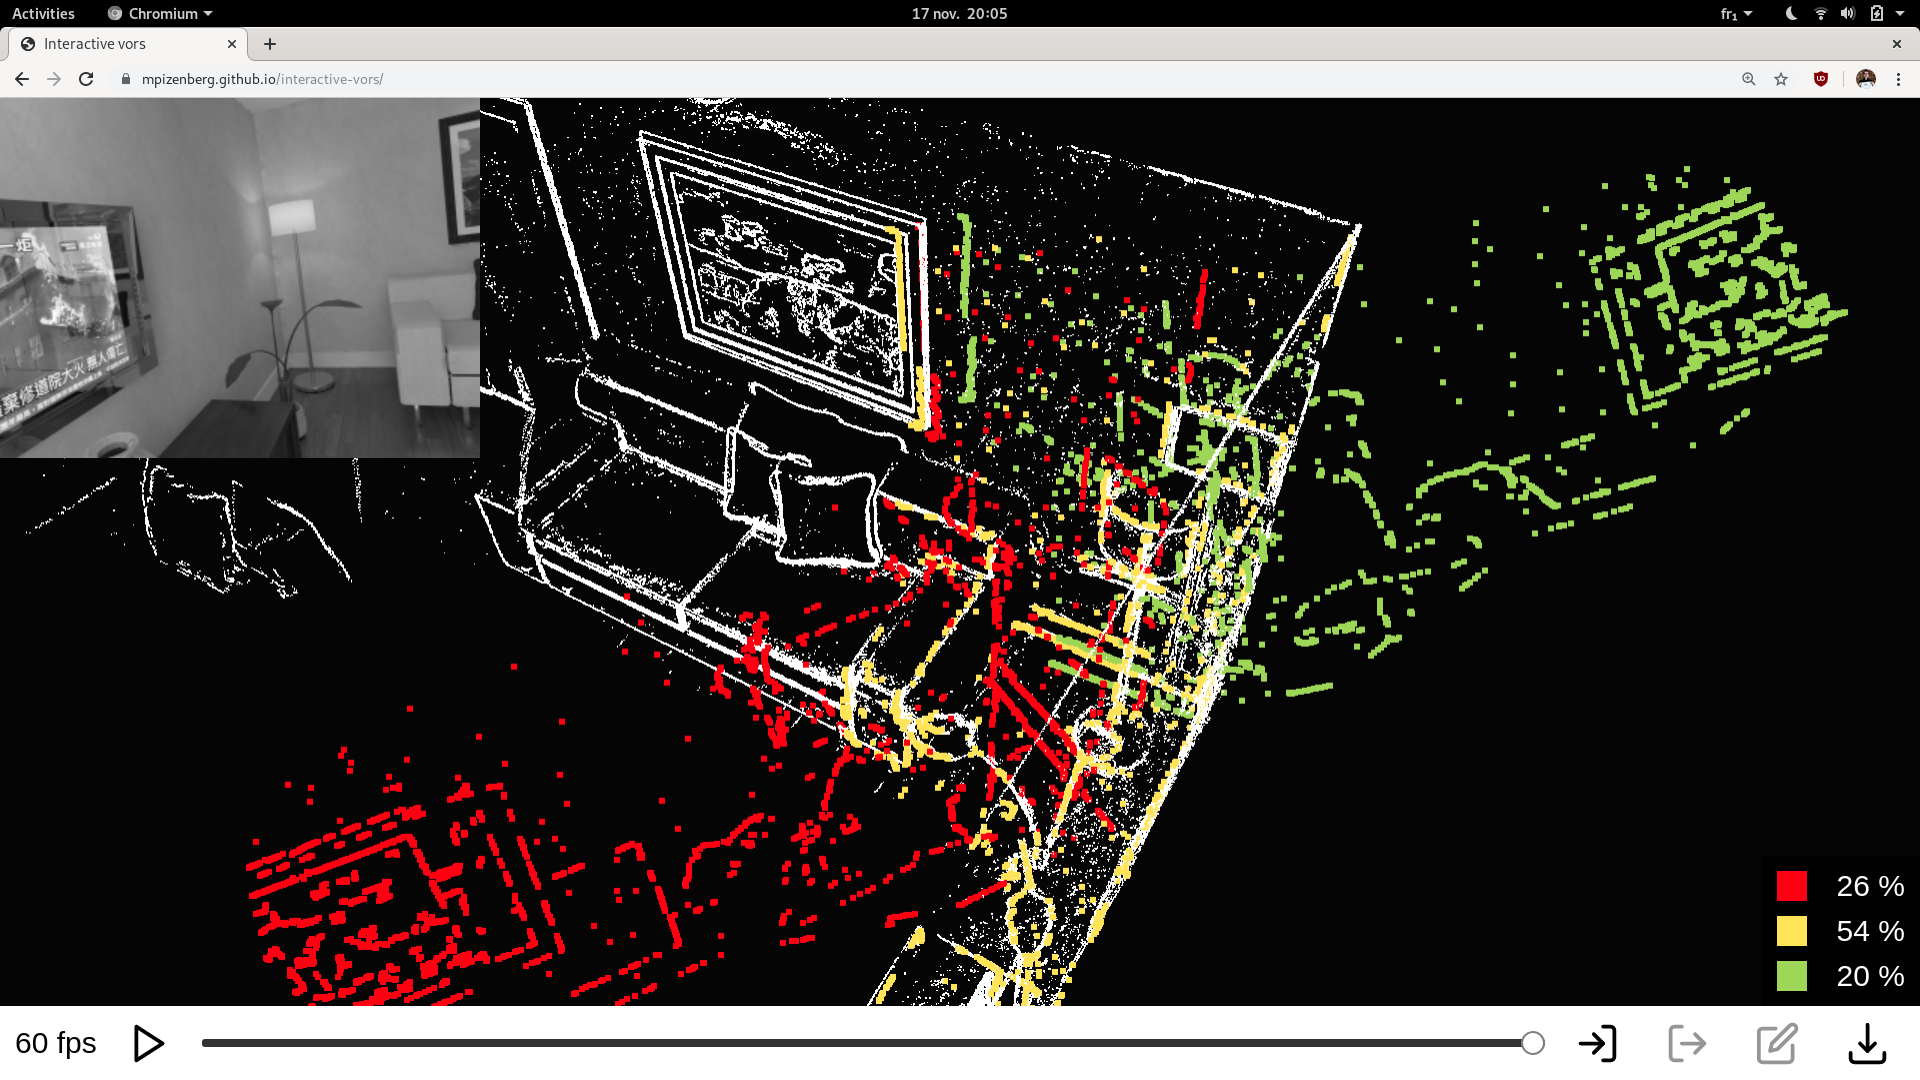
\includegraphics[width=\linewidth]{assets/img/p3p-two.png}
	\caption{Visualization of potential poses for the second keyframe.
	The misaligned attempt at direct image alignment is presented in red.
	Two potential P3P poses are colored in yellow and green.
	An estimation of the probability of each pose to be correct is
	provided in the lower right corner of the visualization canvas.}%
	\label{fig:p3p-two-poses}
\end{figure}

\section{Conclusion}%
\label{sec:vors-ccl}

In this chapter, we presented VORS,
the first complete direct visual odometry algorithm in Rust.
We have paid particular attention to simplicity,
and reduction of parameters in all the steps of the algorithm,
such as for the sparse candidate points selection.
Then, by comparing its precision to other available algorithms,
we demonstrated that VORS achieves state of the art odometry precision on RGB-D datasets,
especially for synthetic data, presenting less outliers to our modelization.
Finally, we presented ``Interactive VORS'',
our interactive Web application, based on the compilation of VORS to WebAssembly.
It provides easy access to visual odometry, directly in a browser,
with interaction in multiple modalities.
A one-dimensional navigation along the temporal axis is provided by a timeline
while three-dimensional space navigation is possible with the point cloud visualization.
We implemented correction of drifts in conditions where loops are present in the sequence.
In general, our goal was to showcase the potential of interactive Web applications
to better understand the huge amount of data generated by visual odometry,
and eventually offer methods to correct automatic results with guided human intervention.
